\documentclass[10pt]{beamer}
\usepackage[latin1]{inputenc}
\usepackage{amsmath}
\usepackage{amsfonts}
\usepackage{amssymb}
\usepackage{makeidx}
\usepackage{graphicx}
\usetheme{Madrid}
\usepackage{tikz}
%%%<
%\usepackage{verbatim}
%\usepackage[active,tightpage]{preview}
%\PreviewEnvironment{center}
%\setlength\PreviewBorder{10pt}%
%%%%>
\usetikzlibrary{arrows}
\usetikzlibrary{automata}
\usetikzlibrary{positioning}


% Defines a `datastore' shape for use in DFDs.  This inherits from a
% rectangle and only draws two horizontal lines.
\makeatletter
\pgfdeclareshape{datastore}{
  \inheritsavedanchors[from=rectangle]
  \inheritanchorborder[from=rectangle]
  \inheritanchor[from=rectangle]{center}
  \inheritanchor[from=rectangle]{base}
  \inheritanchor[from=rectangle]{north}
  \inheritanchor[from=rectangle]{north east}
  \inheritanchor[from=rectangle]{east}
  \inheritanchor[from=rectangle]{south east}
  \inheritanchor[from=rectangle]{south}
  \inheritanchor[from=rectangle]{south west}
  \inheritanchor[from=rectangle]{west}
  \inheritanchor[from=rectangle]{north west}
  \backgroundpath{
    %  store lower right in xa/ya and upper right in xb/yb
    \southwest \pgf@xa=\pgf@x \pgf@ya=\pgf@y
    \northeast \pgf@xb=\pgf@x \pgf@yb=\pgf@y
    \pgfpathmoveto{\pgfpoint{\pgf@xa}{\pgf@ya}}
    \pgfpathlineto{\pgfpoint{\pgf@xb}{\pgf@ya}}
    \pgfpathmoveto{\pgfpoint{\pgf@xa}{\pgf@yb}}
    \pgfpathlineto{\pgfpoint{\pgf@xb}{\pgf@yb}}
 }
}
\makeatother
\tikzset{
    state/.style={
           rectangle,
           rounded corners,
           draw=black, very thick,
           minimum height=2em,
           inner sep=2pt,
           text centered,
           },
}	


\title[Speaker recognition]{Statistical Learning and Applications: M2 project\\
 Speaker Recognition}
\author{Antoine Plet\\
Thomas Sibut-Pinote}
\institute{ENS de Lyon}
\logo{
\includegraphics[height=5mm]{logo.png}}

\begin{document}
\begin{frame}
\maketitle
\end{frame}


\begin{frame}{General scheme of SVM classification}
\begin{figure}[scale=0.1]
\centering
\label{schema}
\caption{Summary}
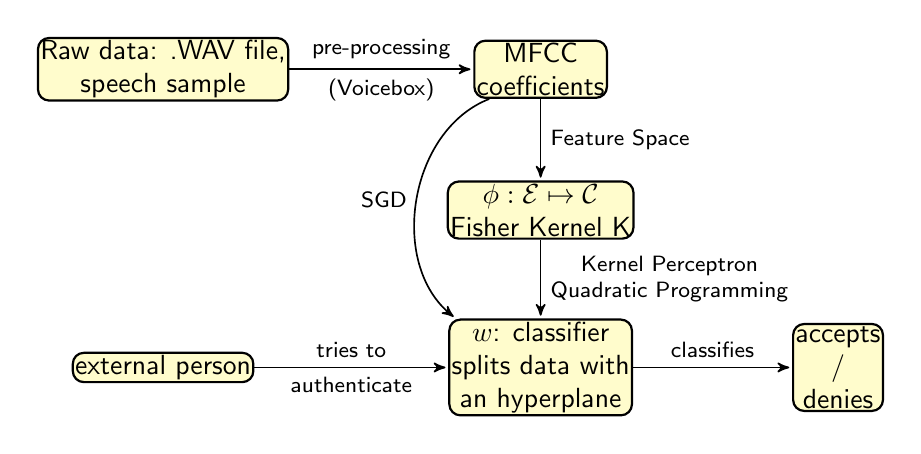
\begin{tikzpicture}[
  font=\sffamily,
  every matrix/.style={ampersand replacement=\&,column sep=2cm,row sep=1cm},
  source/.style={draw,thick,rounded corners,fill=yellow!20,inner sep=.03cm},
  process/.style={draw,thick,circle,fill=blue!20},
  sink/.style={source,fill=green!20},
  datastore/.style={draw,very thick,shape=datastore,inner sep=.07cm},
  dots/.style={gray,scale=2},
  to/.style={->,>=stealth',shorten >=1pt,semithick,font=\sffamily\footnotesize},
  every node/.style={align=center}]

  % Position the nodes using a matrix layout
  \matrix{
    \node[source] (hisparcbox) {Raw data: .WAV file,\\ speech sample};
      \& \node[source] (daq) {MFCC \\coefficients}; \& \\

    \& \node[source] (buffer) {$\phi: \mathcal{E} \mapsto \mathcal{C}$\\ Fisher Kernel K}; \& \\

    \node[source] (storage) {external person};
      \& \node[source] (monitor) {$w$: classifier 
      \\ splits data with\\ an hyperplane};
      \& \node[source] (datastore) {accepts\\/\\denies}; \\
  };

  % Draw the arrows between the nodes and label them.
  \draw[to] (hisparcbox) -- node[midway,above] {pre-processing}
     node[midway,below] {(Voicebox)} (daq);
  \draw[to] (daq) -- node[midway,right] {Feature Space} (buffer);
  \draw[to] (buffer) --
      node[midway,right] {Kernel Perceptron\\Quadratic Programming} (monitor);
%  \draw[to] (monitor) to[bend right=50] node[midway,above] {events}
%      node[midway,below] {level 1} (storage);
  \draw[to] (storage) to node[midway,above] {tries to}
      node[midway,below] {authenticate} (monitor);
  \draw[to] (monitor) -- node[midway,above] {classifies}
       (datastore);
  \draw[to] (daq) to[bend right=60] node[midway,left] {SGD}
             (monitor);
\end{tikzpicture}
\end{figure}
\end{frame}

\begin{frame}{Data and preprocessing}
\begin{block}{Starting point}
\begin{itemize}
\item We recorded ourselves and a few other people..
\item ..and we took a recording of a famous politician and someone trying to imitate him. %commentaire oral: after all, that's what we want to fight!!
\item They were all in .WAV format
\end{itemize}
\end{block}

\begin{block}{Pre-processing}
We computed MFCC coefficients from those files: Discrete Cosine Transform + some other functions which have proven to work well in the past.
\end{block}
\end{frame}

\begin{frame}{Stochastic gradient descent}
\begin{block}{Parameter of SGD}
  $f_{obj}(w) := \frac{1}{2} \|w\|^2 + C\displaystyle\sum\limits_{i=1}^{n}l_i(w)$ with $l_i(w) := \mathrm{hinge}(y_i (w \cdot x_i + b))$
\end{block}

\begin{block}{What we got}
Our final program:
\begin{itemize}
  \item Input: data set, name, bunch of C values
  \item Output: a function: .wav $\rightarrow \{0, 1\}$ 
\end{itemize}
\end{block}
\end{frame}


\begin{frame}{General scheme of SVM construction}
\begin{figure}
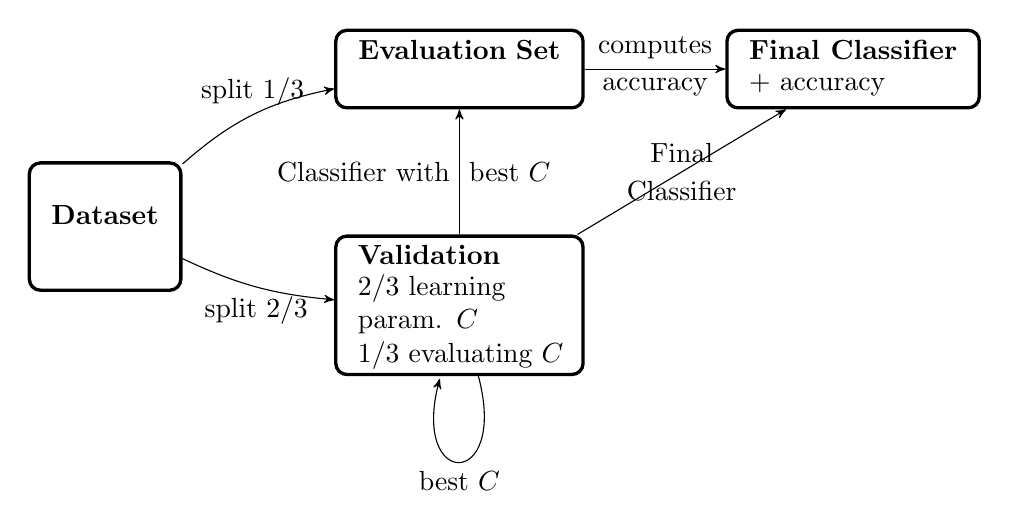
\begin{tikzpicture}[->,>=stealth']

 % Position of QUERY 
 % Use previously defined 'state' as layout (see above)
 % use tabular for content to get columns/rows
 % parbox to limit width of the listing
 \node[state] (QUERY) 
 {\begin{tabular}{l}
  \\
  \textbf{Dataset}\\
  \\[0.6em]

 \end{tabular}};
  
 % State: ACK with different content
 \node[state,    	% layout (defined above)
  text width=3cm, 	% max text width
  yshift=2cm, 		% move 2cm in y
  right of=QUERY, 	% Position is to the right of QUERY
  node distance=4.5cm, 	% distance to QUERY
  anchor=center] (ACK) 	% posistion relative to the center of the 'box'
 {%
 \begin{tabular}{l} 	% content
  \textbf{Evaluation Set}\\
  \parbox{2.8cm}{}
 \end{tabular}
 };
 
 % STATE QUERYREP
 \node[state,
  below of=ACK,
  yshift=-2cm,
  anchor=center,
  text width=3cm] (QUERYREP) 
 {%
 \begin{tabular}{l}
  \textbf{Validation}\\
  \parbox{2.8cm}{$2/3$ learning param. $C$\\
  $1/3$ evaluating $C$}
 \end{tabular}
 };

 % STATE EPC
 \node[state,
  right of=ACK,
  node distance=5cm,
  anchor=center] (EPC) 
 {%
 \begin{tabular}{l}
  \textbf{Final Classifier}\\
  \parbox{2cm}{+ accuracy}
 \end{tabular}
 };

 % draw the paths and and print some Text below/above the graph
 \path (QUERY) 	edge[bend left=15]  node[anchor=south,above]{split $1/3$} (ACK)
 (QUERY)     	edge[bend right=10] node[anchor=south,below]{split $2/3$} (QUERYREP)
 (ACK)       	edge                node[anchor=south,above]{computes}
 									node[anchor=south,below]{accuracy} (EPC)
 (QUERYREP)     edge                node[anchor=left,above]{Final} 
 									node[anchor=north,below]{Classifier}          (EPC)   
 (QUERYREP)  	edge[loop below]    node[anchor=north,below]{best $C$} (QUERYREP)
 (QUERYREP)  	edge                node[anchor=left,left]{Classifier with}
 	                                node[anchor=left,right]{best $C$} (ACK);


\end{tikzpicture}
\caption{How we compute the classifier for SGD}
\end{figure}
\end{frame}

\begin{frame}{Stochastic gradient descent: validation}
\begin{figure}[!h]
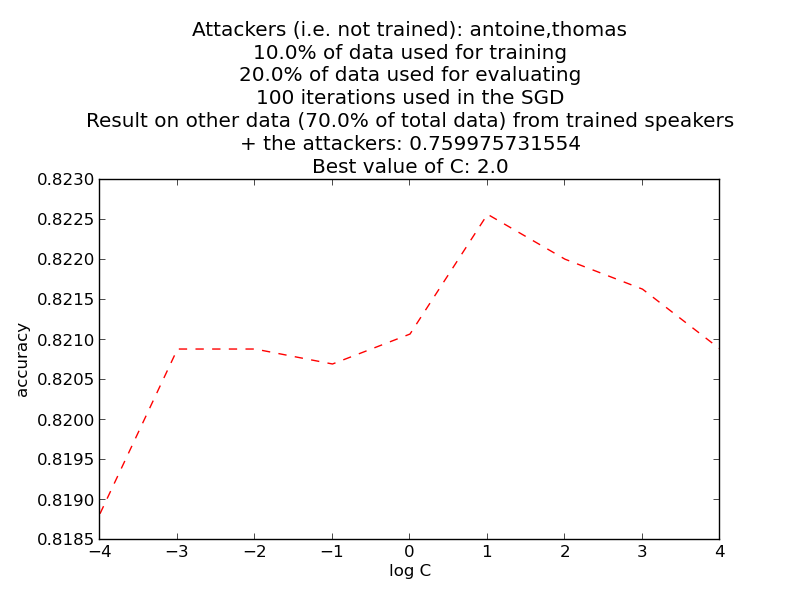
\includegraphics[width=0.7\textwidth]{../bestC}
\end{figure}
\end{frame}

\begin{frame}{Fisher kernel}
\begin{block}{The Fisher Kernel}
The Fisher Kernel is based on a generative model, in our case a Gaussian Mixture model.\\
The vectors considered are packets of frames. If $x$ is a vector, the Fisher score is
\[u_{\bar{x}} = \nabla_{\theta} \log p (\bar{x} | \theta) \]
and the Fisher Kernel is then computed by
\[K(\bar{x}_i,\bar{x}_j) = u_{\bar{x}_i}^{T} I(\theta)^{-1} u_{\bar{x}_j}\]
where $I(\theta)$ is approximated well enough by the identity matrix in our case.
\end{block}
\end{frame}

\begin{frame}{Kernel perceptron}
We first used the Fisher kernel with the kernel perceptron algorithm.\\

\begin{figure}[!h]
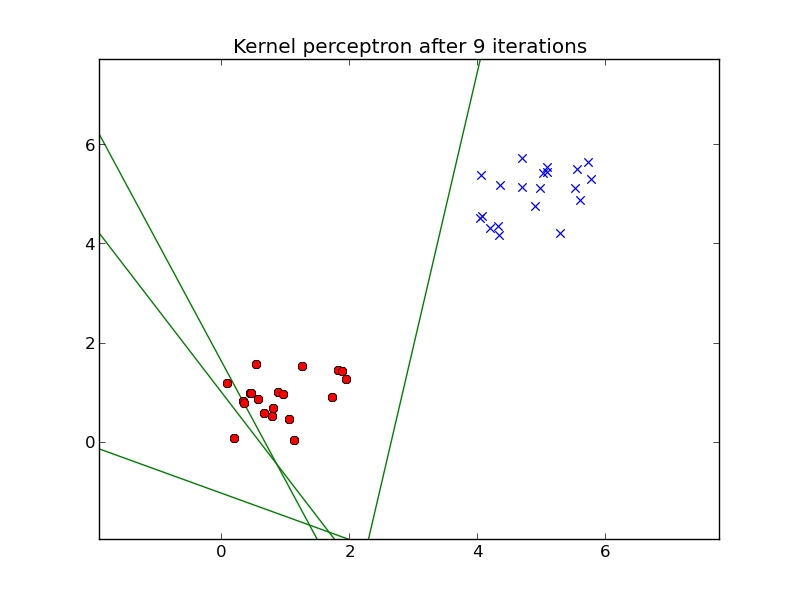
\includegraphics[width=0.65\textwidth]{../rapport/img/kp_pdf}
\caption{Kernel perceptron unrolled (without kernel)}\label{/test_kp}
\end{figure}
\end{frame}

\begin{frame}{Kernel perceptron: validation}
Some convergence problems are preventing us from this step for now. The algorithm needs too many iterations to stop and get stopped by the bound on the number of iterations giving bad results when it occurs. The optimization with such an issue is not reliable.
\end{frame}

\begin{frame}{Quadratic programming}
We then used quadratic programming with Matlab to implement a new classifier.
\begin{block}{Dual problem}
\begin{equation}
  \left\{
    \begin{array}{lll}
      \displaystyle\min_{\alpha}& \frac{1}{2} \alpha^\top  G \alpha - e^\top  \alpha&\\
      \mbox{avec} &y^\top  \alpha = 0 &\\
      \mbox{et} &0 \leq \alpha_i \leq C,& i=1 \dots n \\
    \end{array}
  \right.
\end{equation}
\end{block}
\end{frame}

\begin{frame}{Quadratic programming: validation}
We wanted to optimize the number of Gaussians in the generative model.
\begin{figure}[!h]
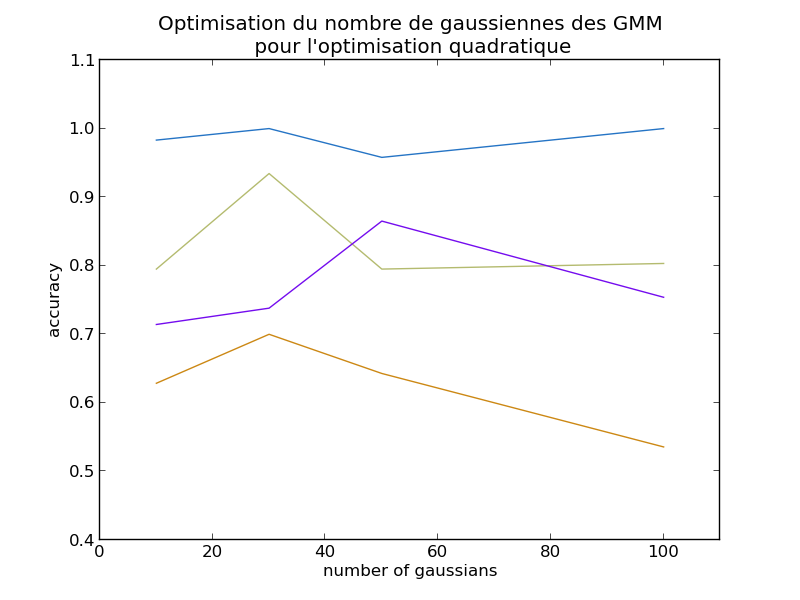
\includegraphics[width=0.5\textwidth]{../rapport/img/opt_qp_pdf}
\caption{Variation de la pr�cision en fonction du nombre de gaussiennes}\label{opt_qp}
\end{figure}
\end{frame}

\begin{frame}{Final tests}
Finally, we evaluate those methods on a famous personality and an imitator. The aim is to learn the personality without the imitator in the data and then test both the personality and the imitator
\begin{itemize}
  \item With the SGD method, we got 1 false positive out of 13 tests and 1 false negative out of 14 tests: good
\end{itemize}
\end{frame}

\begin{frame}{Conclusion}
  \begin{itemize}
    \item We implemented various classifiers based on SVM and compared them with one another;
    \item We implemented the SGD method;
    \item We can successfully classify the speaker in most cases, even when he/she is imitating someone;
    \item In the future we may want to average the results over more experiments.
  \end{itemize}
\end{frame}

\begin{frame}
\fontsize{15}{17}\selectfont
\begin{center}
Thank you for your attention. \\
\vspace{.4in}
Any questions?
\end{center}
\end{frame}

\end{document}